\documentclass[11pt]{article}

% ARR/ACL template. Switch [review] to [final] once accepted.
\usepackage[review]{acl}

\usepackage[T1]{fontenc}
\usepackage[utf8]{inputenc}
\usepackage{booktabs}
\usepackage{graphicx}
\usepackage[expansion=false]{microtype}

\title{Decontaminated by Whose Standard?\\
Label-Free Measurement of Decontamination Filter Error}

\begin{document}
\maketitle

\begin{abstract}
Open post-training projects routinely state that their training data has been
decontaminated against public benchmarks, and readers treat that statement as
meaning roughly the same thing across projects. Reimplementing five such filters
from their released source and running all of them over one corpus against one
benchmark suite, we find they flag between $0\%$ and $27.5\%$ of the same items.
Disagreement alone, however, invites the reply that different tools simply sit at
different thresholds.

Our main contribution settles that. Benchmark items published \emph{after} a
corpus was assembled cannot appear in it, so any flag against them is a false
positive by construction, identifiable without annotation. Using competition sets
held after the corpus cutoff as a negative control, we find the two filters that
detect anything are wrong about more than a tenth of what they report:
$12.9\%$ and $11.1\%$ false positives, replicated at $6.2\%$ and $6.9\%$ on a
second, independent corpus. That is not a threshold preference but a measured
error rate, and it is stable in proportion across a $31\times$ range of corpus
size. We verify the control assumption directly rather than assuming it, and trace
every error to the stock phrasing of competition mathematics rather than to leaked
content.

Because the control is label-free, it also tunes. Applied as a sweep it shows that
$n$-gram size trades sensitivity without buying precision, and that the
best-performing method in our comparison ships a default threshold that disables
it.
\end{abstract}

\section{Introduction}

A benchmark score is evidence of capability only if the benchmark was held out.
Open post-training projects generally assert that it was: model cards and papers
state that training data was decontaminated against the suites on which results
are reported. Readers, and downstream leaderboards, treat those assertions as
comparable.

They are comparable only if the underlying procedures agree. This paper asks
whether they do, and finds that they do not, by a wide margin.

We take five decontamination filters that ship with real released datasets,
reimplement each from its own source, and apply all five to a single corpus
against a single benchmark suite. The spread is not subtle. On $100{,}000$
training documents and $502$ benchmark items, the filters flag $0$, $0$, $6$,
$127$ and $138$ items respectively. Whether a benchmark problem counts as
contaminated is, in practice, a function of which tool was run.

That much is only an observation, and it has an easy dismissal: different tools
are tuned differently, and a spread of thresholds is what one would expect.
Establishing that filters disagree does not establish that any of them is
\emph{wrong}.

Answering that has previously required human adjudication, which is expensive and
unreliable at exactly the boundary cases that decide it. We propose a cheaper and
more decisive test. Competition mathematics produces new benchmarks continuously
and with known dates. An item published after a corpus was assembled cannot be
present in it. Any filter that flags such an item has made an error that requires
no judgement to identify, and the dismissal does not survive it, because a
threshold choice does not explain why half of what a filter reports is wrong.

Using this construction we contribute:

\begin{itemize}
\item A label-free method for measuring decontamination false-positive rates,
using post-cutoff benchmarks as a negative control (\S\ref{sec:control}), with the
control assumption tested rather than assumed (\S\ref{sec:validate}).
\item Measured error rates of $12.9\%$ and $11.1\%$ for the two filters that
detect anything, replicated at $6.2\%$ and $6.9\%$ on an independent corpus
(\S\ref{sec:second}), and stable in proportion across a $31\times$ range of corpus
size (\S\ref{sec:scale}).
\item A mechanistic account of those errors: all of them arise from a small set of
conventional competition-mathematics phrases (\S\ref{sec:why}).
\item A direct comparison of five published decontamination filters, each run from
its released implementation on identical inputs (\S\ref{sec:disagree}).
\item A tuning procedure built on the control set, showing that $n$-gram size is a
sensitivity parameter rather than a precision parameter, and that fuzzy
whole-string matching dominates $n$-gram matching at every operating point we
measured (\S\ref{sec:tune}).
\end{itemize}

We emphasise at the outset that this is not a finding that any project was
careless. Every filter we study does what its authors implemented. The problem is
that one word describes procedures measuring different things.

\section{Related Work}

Work on benchmark contamination divides into detection from the model side and
inspection from the data side. Model-side methods ask whether a trained model
shows evidence of having seen an evaluation item, through membership inference,
loss-based tests, or exchangeability arguments \citep{oren2024}. A systematic
review of 55 such studies finds that no method is reliable across contamination
regimes \citep{gemreview}, and \citet{reliabilitygap} report that across 335
evaluations of three leading paradigms only 60\% yield correct outcomes,
concluding explicitly that statistical detection cannot yet replace transparent
data provenance. \citet{detectable} give an information-theoretic account of why,
showing that detectability scales with prevalence and sample size such that
audit-scale samples are underpowered by one to two orders of magnitude.
Contamination detection in reasoning models is separately fragile
\citep{fragility}, and detectors built on LLM judges inherit contamination
problems of their own \citep{preferenceleakage, judgerobustness}.

This paper works on the provenance side that such conclusions point toward: the
training corpus is public, so overlap can be inspected directly. Prior data-side
work has generally audited one corpus with one detector and reported a
contamination rate \citep{sainz2023}, and paraphrase-based evasion is known to
defeat surface matching \citep{yang2023rephrase}. Our question is prior to those.
Before asking how contaminated a corpus is, we ask whether the quantity is well
defined, given that the procedures in use disagree. Recent work pursuing
statistical guarantees for detection \citep{controllable} is complementary: it
assumes the target quantity is fixed, which is what we test.

A parallel literature examines the reliability of audit pipelines themselves.
\citet{auditingtheaudit} give a five-class taxonomy of pipeline failures in
perturbation-based validity audits, and \citet{reliabilitygap} study distribution
shift and scale as limits on model-side detection. Both concern audits of models.
To our knowledge no prior work runs multiple published decontamination
\emph{implementations} over a common corpus and reports the divergence in what
they flag.

The artifacts we study are s1 \citep{s1}, T\"{u}lu~3 \citep{tulu3}, OpenThoughts
and OpenThoughts3 \citep{openthoughts}, and Olmo~3 \citep{olmo3}, whose data and
decontamination code are all public. Our benchmarks come from OlymMATH
\citep{olymmath} and MathArena \citep{matharena}.

\section{The Filters}
\label{sec:filters}

We reimplemented each filter from its released source, or compiled and ran the
released binary where one exists. Table~\ref{tab:filters} summarises what each
does, which in two cases differs from what its paper describes.

\begin{table*}[t]
\centering
\small
\begin{tabular}{llll}
\toprule
\textbf{Filter} & \textbf{Method} & \textbf{Tokenizer} & \textbf{Params from} \\
\midrule
s1 & any shared 8-gram & whitespace, lowercased & code \\
Tulu 3 & coverage fraction over Elasticsearch & spaCy / ES analyzer & paper prose only \\
OpenThoughts-114K & \texttt{fuzz.ratio} $\geq 95$ & none (raw strings) & code \\
OpenThoughts3 & any shared 13-gram & \texttt{Qwen/Qwen2-7B-Instruct} & code \\
\texttt{decon} (Olmo 3) & 5-gram detect, then cluster scoring & \texttt{cl100k} & code \\
\bottomrule
\end{tabular}
\caption{The five filters as implemented rather than as described. Two points
deserve emphasis: OpenThoughts-114K performs no $n$-gram matching at all, and
Tulu 3's two governing parameters have no defaults anywhere in its released code.}
\label{tab:filters}
\end{table*}

Three observations follow from reading the sources.

\paragraph{The filters do not implement the same kind of test.}
Three are single-stage: a match on any shared $n$-gram, or a whole-string
similarity above a cutoff. \texttt{decon} is two-stage, generating candidates by
5-gram overlap and accepting them only if a weighted score exceeding $0.8$
survives cluster expansion. Tulu 3 computes a coverage fraction over documents
retrieved by Elasticsearch, so its recall is bounded by retrieval.

\paragraph{The tokenizer is where single-stage filters diverge most.}
s1 splits on whitespace after lowercasing; OpenThoughts3 hardcodes a model
tokenizer. Eight whitespace tokens and eight model tokens describe very different
amounts of text, so the same nominal $n$ means different things.

\paragraph{In two cases the released code and the written description do not
line up.} These are observations about artifacts, not about anyone's conduct, and
in both cases there is a benign reading.

The decontamination code released with OpenThoughts-114K contains no $n$-gram
logic at all: it calls \texttt{process.extract} with \texttt{fuzz.ratio} at a
cutoff of $95$ on raw strings. A 13-gram path does exist in the same repository,
but under OpenThoughts3, a later and separate release. A reader who takes
``13-gram'' as describing the 114K artifact would be mistaken, though the
description is accurate for the artifact it belongs to. Distinguishing the two
requires reading the repository.

T\"{u}lu~3's \texttt{-{}-ngram\_size} and \texttt{-{}-match\_threshold} are declared
without defaults and fall through as \texttt{None}, so the ``8-gram'' and
``$>50\%$ coverage'' that its paper states are not recoverable from the code. The
values were presumably supplied at run time by a driver that was not released.
Either way a third party cannot reproduce the configuration, so we mark T\"{u}lu~3's
parameters as prose-derived throughout and treat its numbers accordingly.

Neither observation implies the filters were applied carelessly. Both illustrate
the paper's point: what ``decontaminated'' denotes is fixed by an implementation,
and an implementation is only as recoverable as what was released alongside it.

\section{Label-Free Evaluation via Temporal Controls}
\label{sec:control}

Determining whether a flagged item is genuinely contaminated normally requires
human adjudication, which is costly and unreliable at the boundary cases that
matter most.

Competition mathematics offers an alternative. New problem sets are released
continuously, at publicly known dates. For a corpus assembled at time $t$, any
benchmark published after $t$ cannot be contained in it, whatever a filter
reports. Flags against such items are false positives by construction: not
estimates, not adjudications, but logical impossibilities.

This yields a two-group design. A \textbf{measurement set} of benchmarks
published before the corpus cutoff, where flags may be correct or incorrect, and
a \textbf{control set} published after it, where every flag is wrong. The control
set gives a false-positive rate directly, with no annotation, and can be
recomputed for any corpus whose assembly date is known.

The design has one requirement: the cutoff must be established independently of
the filters being evaluated. We use the corpus's public release date as an upper
bound, and exclude benchmarks falling near it.

\subsection{Testing the assumption}
\label{sec:validate}

That upper bound is load-bearing, and Dolci is a remix of separately curated
corpora, so in principle a component could postdate the release of the whole. We
therefore test it rather than assert it. A benchmark item genuinely present in a
corpus shares long spans with some training document; a coincidental match shares
only short ones. For every benchmark item we computed the longest $n$ for which it
shares an $n$-gram with any training document.

\begin{table}[h]
\centering
\small
\begin{tabular}{lrr}
\toprule
\textbf{Longest match} & \textbf{Measure} & \textbf{Control} \\
 & (502) & (280) \\
\midrule
no match      & 375 & 244 \\
$\geq 8$      &  91 &  25 \\
$\geq 10$     &  29 &   9 \\
$\geq 13$     &   7 &   1 \\
$\geq 15$     &   0 &   1 \\
\bottomrule
\end{tabular}
\caption{Longest word $n$-gram each benchmark item shares with the corpus.}
\label{tab:validate}
\end{table}

No control item matches at a length that would indicate presence, and inspection
of the five longest control spans finds no problem content at all. The longest,
at $n{=}15$, is \emph{``where $m$ and $n$ are relatively prime positive integers,
find $m+n$''}, the conventional closing of an AIME problem. The others are
\emph{``is not divisible by the square of any prime''} and \emph{``reads the same
from left to right as from right''}. These are genre conventions, not leaked text.

The longest single shared span anywhere in this study therefore belongs to an item
that provably postdates the corpus, and consists entirely of boilerplate. That is
both the assumption discharged and the clearest single illustration of the
mechanism analysed in \S\ref{sec:why}.

\section{Experimental Setup}

\paragraph{Corpus.}
\texttt{allenai/Dolci-Think-SFT-32B}, the post-training data for Olmo 3
($2{,}253{,}684$ examples). Olmo 3 was announced 20 November 2025, so we treat the
corpus as closed by roughly October 2025. We use a $100{,}000$-document sample for
the main results and up to $390{,}000$ for the scaling analysis. Filters read the
first user turn of each example, the field their own implementations target.

Dolci is a remix of separately curated corpora. In our sample the largest slices
are OpenThoughts3 Math ($34{,}835$), Python Algorithms ($21{,}090$), Persona
Precise IF ($10{,}089$), Nemotron Code ($5{,}232$) and SYNTHETIC-2 ($4{,}914$).
Each was decontaminated, if at all, by whoever assembled it.

\paragraph{Measurement set (502 items).}
OlymMATH (200) plus ten MathArena competitions held on or before September 2025:
Apex 2025, the Apex shortlist, SMT 2025, CMIMC 2025, BRUMO 2025, AIME 2025,
HMMT February 2025, both AIME 2024 papers, and HMMT February 2024.

\paragraph{Control set (280 items).}
Eight MathArena sets from January to August 2026: AIME 2026, HMMT February 2026,
USAMO 2026, three ArXivMath sets and two BrokenArXiv sets. All postdate the
corpus by at least three months.

\section{Filters Disagree}
\label{sec:disagree}

\begin{table}[t]
\centering
\small
\setlength{\tabcolsep}{3.5pt}
\begin{tabular}{lrr}
\toprule
\textbf{Filter} & \textbf{Measure} & \textbf{Control} \\
 & (502) & (280) \\
\midrule
\texttt{decon} & 0 (0.0\%) & 0 (0.0\%) \\
fuzzy, cutoff 95 & 0 (0.0\%) & 0 (0.0\%) \\
T\"{u}lu 3 coverage & 6 (1.2\%) & 0 (0.0\%) \\
s1 8-gram & 127 (25.3\%) & 36 (12.9\%) \\
OpenThoughts3 13-gram & 138 (27.5\%) & 31 (11.1\%) \\
\bottomrule
\end{tabular}
\caption{Benchmark items flagged, $100{,}000$ Dolci documents. Every control-set
flag is a false positive by construction.}
\label{tab:main}
\end{table}

Table~\ref{tab:main} gives the central result. The filters separate into two
groups with nothing between them. Three flag almost nothing and are never wrong.
Two flag a quarter of the benchmark and are wrong about more than a tenth of it.
There is no shared standard for where on this range the word ``decontaminated''
should sit.

Agreement between them is close to absent. Of the $201$ items ($40.0\%$ of the
benchmark) flagged by at least one filter, $133$ ($66.2\%$; $95\%$ CI
$[59.6, 72.6]$ by bootstrap over benchmark items, $B{=}10{,}000$) are flagged by
\emph{exactly one}. Two items reach three of five, and none reaches four. The
highest pairwise Jaccard overlap is $0.318$, between the two $n$-gram filters;
every other pair falls below $0.05$.

\texttt{decon}'s zero is robust rather than marginal: it returns zero at its
default score threshold of $0.8$, zero at $0.6$, a single contaminated document at
$0.4$, and $646$ only at $0.2$, a quarter of the default.

\paragraph{A caution about partial reimplementation.}
Our first attempt at \texttt{decon} implemented only its candidate-generation
stage, a 5-gram match over \texttt{cl100k} tokens. That version flagged $199$ of
$200$ items. The real binary flags none. Reporting the approximation would have
inverted the result and misrepresented the tool. A filter is its whole pipeline,
and two-stage filters cannot be approximated by their first stage.

\section{Measured False-Positive Rates}

Both $n$-gram filters flag items that cannot be in the corpus: $12.9\%$ of the
control set for s1 ($95\%$ CI $[9.3, 16.8]$) and $11.1\%$ for OpenThoughts3
($[7.5, 15.0]$), against measurement rates of $25.3\%$ $([21.5, 29.1])$ and
$27.5\%$ $([23.5, 31.7])$. Intervals are bootstrap over benchmark items,
$B{=}10{,}000$; the control set has $280$ items, so these carry roughly four
points of uncertainty and both nonetheless exclude zero by a wide margin.

Subtracting the control rate from the measurement rate leaves roughly $12.4\%$ and
$16.4\%$ as estimates of genuine detection, meaning about half of s1's reported
signal is noise. The three conservative filters have no false positives and almost
no true positives.

\section{The Error Rate Is Intrinsic}
\label{sec:scale}

\begin{figure*}[t]
\centering
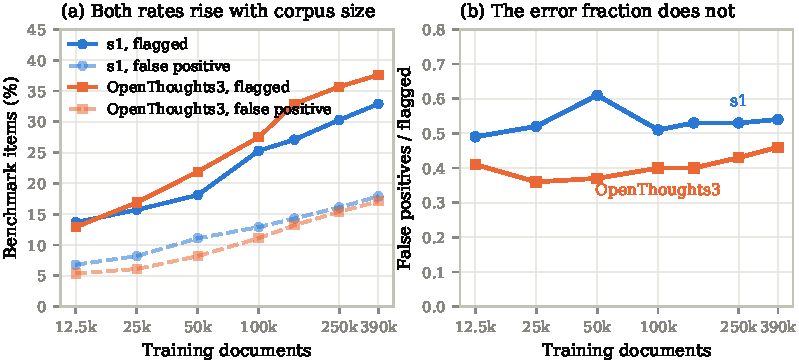
\includegraphics[width=\textwidth]{figures/scaling.pdf}
\caption{Across a $31\times$ range of corpus size, both the flag rate and the
false-positive rate roughly double (a), while the fraction of each filter's
output that is provably wrong stays flat (b). The error is a property of the
method, not of how much data it is given.}
\label{fig:scaling}
\end{figure*}

A single-corpus measurement invites the objection that it may not survive
scaling. It does not need to: Figure~\ref{fig:scaling} shows the error fraction
is invariant. Across seven corpus sizes from $12{,}500$ to $390{,}000$
documents, absolute rates roughly double, for false positives as much as for
detections, while the \emph{proportion} of error stays flat. s1's false-positive
fraction runs $0.49$, $0.52$, $0.61$, $0.51$, $0.53$, $0.53$, $0.54$;
OpenThoughts3's runs $0.41$, $0.36$, $0.37$, $0.40$, $0.40$, $0.43$, $0.46$,
drifting upward, so that filter becomes relatively worse as the corpus grows.

The corrected signal does grow, from $7.0\%$ to $12.8\%$ for s1 and $7.6\%$ to
$19.7\%$ for OpenThoughts3, so real overlap is found beneath the noise. It is
outnumbered at close to a fixed ratio, and no choice of corpus size changes that.

\texttt{fuzz.ratio} returns zero at every scale up to $250{,}000$ and one item at
$390{,}000$; \texttt{decon} returns zero throughout. The architectural
disagreement between whole-string and $n$-gram matching is therefore
scale-invariant, and is the more portable of our two findings.

\section{The Errors Are Not Specific to One Corpus}
\label{sec:second}

To test whether the false-positive rate is a property of these filters or of
Dolci, we repeated the measurement on an independent corpus: the T\"{u}lu~3 SFT
mixture's mathematics subset, released November 2024. The date split moves with
the corpus. Every 2025 competition now postdates it, so the control side grows to
$722$ items and only the three 2024 competitions remain as a measurement set.

\begin{table}[h]
\centering
\small
\setlength{\tabcolsep}{3.5pt}
\begin{tabular}{lrr}
\toprule
\textbf{Filter} & \textbf{Detect} & \textbf{False pos.} \\
 & (60) & (722) \\
\midrule
s1 8-gram             & 2 (3.3\%) & 45 (6.2\%) \\
OpenThoughts3 13-gram & 1 (1.7\%) & 50 (6.9\%) \\
fuzzy, cutoff 95 & 0 (0.0\%) & 0 (0.0\%) \\
T\"{u}lu 3 coverage         & 0 (0.0\%) & 0 (0.0\%) \\
\bottomrule
\end{tabular}
\caption{The same filters on the T\"{u}lu~3 SFT math subset, $100{,}000$ documents.}
\label{tab:second}
\end{table}

Both $n$-gram filters again flag items that cannot be present, at $6.2\%$ and
$6.9\%$. The phenomenon is therefore a property of the method rather than of
Dolci. Its magnitude is not: the rate here is roughly half what it is on Dolci,
so a false-positive rate must be measured per corpus and cannot be carried over.

We deliberately draw no conclusion about detection on this corpus. Sixty
measurement items give an estimate with a $95\%$ interval of roughly $[0.4, 11.5]$
percent, which cannot be compared meaningfully against the false-positive rate.
The control side is what this corpus is useful for, and it is the larger of the
two.

Incidentally, T\"{u}lu~3's own filter flags nothing in T\"{u}lu~3's own data, which is
what one would expect if it was in fact run.

\section{Why the Errors Happen}
\label{sec:why}

All $36$ of s1's false positives trace to $73$ distinct 8-grams, and none is a
fragment of a leaked problem. They are the conventional phrasing of competition
mathematics: \emph{find the sum of all possible values of} ($166$ documents),
\emph{let a and b be positive integers such} ($67$), \emph{is not divisible by the
square of any} ($67$), \emph{where m and n are relatively prime positive} ($8$
documents, matching $6$ distinct control items).

AIME problems conventionally close by asking for $m+n$ where $m$ and $n$ are
relatively prime; ``not divisible by the square of any prime'' is standard framing
for a radical-form answer. These conventions are shared by every problem of the
type, including problems written months after the corpus was assembled.

This explains the precision ceiling of \S\ref{sec:tune}. Competition mathematics
has a fixed inventory of set phrases eight or more words long, so an eight-word
window can be filled entirely by convention, carrying no problem-specific content.
Increasing $n$ does not escape the problem, because the phrases are themselves
long.

\section{Tuning Without Labels}
\label{sec:tune}

\begin{figure}[t]
\centering
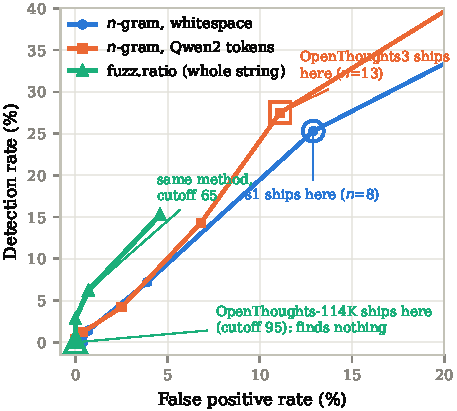
\includegraphics[width=\columnwidth]{figures/frontier.pdf}
\caption{Precision/recall frontier, derived without labels. Rings mark each
project's shipped default. Whole-string fuzzy matching dominates both $n$-gram
families in the low-error region, but the project using it ships a cutoff of
$95$, at which it flags nothing. Points beyond $20\%$ false positives are
omitted; at $n{=}5$ both $n$-gram families flag essentially the whole benchmark.}
\label{fig:frontier}
\end{figure}

Because control-set flags are provably wrong, sweeping a filter's parameters over
both groups yields a precision/recall curve with no annotation anywhere
(Figure~\ref{fig:frontier}).

\paragraph{$n$-gram size is a sensitivity knob, not a precision knob.}
For whitespace tokens the error fraction is pinned near $0.51$ from $n{=}8$ to
$n{=}13$ while detection falls from $25.3\%$ to $1.4\%$: raising $n$ buys no
precision, only insensitivity. At $n{=}15$ detection reaches zero while false
positives persist, so everything found is wrong. Model-token $n$-grams do improve
with $n$, from an error fraction of $1.00$ at $n{=}5$ to $0.40$ at $n{=}13$ and
$0.30$ at $n{=}25$, but reaching a fraction below $0.1$ costs all but $0.4\%$ of
detection.

Notably, s1 (whitespace, $n{=}8$: $25.3\%$ detection, $12.9\%$ error) and
OpenThoughts3 (Qwen, $n{=}13$: $27.5\%$, $11.1\%$) sit at nearly the same
operating point despite sharing no parameters.

\paragraph{The best method ships the worst default.}
Sweeping \texttt{fuzz.ratio} gives $0\%$ detection at its shipped cutoff of $95$,
$2.8\%$ at $70$ with no false positives at all, $6.2\%$ at $65$ with $0.7\%$, and
$15.3\%$ at $60$ with $4.6\%$. At comparable recall this dominates $n$-gram
matching: $6.2\%$ detection at $0.7\%$ error against a whitespace 10-gram's
$7.2\%$ at $3.9\%$, a fivefold difference. The method that performs best in our
comparison is the one whose default disables it, and the remedy is a threshold
roughly thirty points lower.

\section{Contamination Is Concentrated in One Slice}
\label{sec:composition}

Mapping flagged items back to the Dolci source that triggered them shows overlap
is not spread evenly across the remix. Under the OpenThoughts3 filter, which flags
$138$ measurement items, SYNTHETIC-2 supplies $4.9\%$ of our corpus sample and
accounts for $72$ of them, a tenfold enrichment. Nemotron Code supplies $5.2\%$
and accounts for $26$ ($3.6\times$). By contrast OpenThoughts3 Math supplies
$34.8\%$ of the corpus and accounts for $70$ ($1.5\times$), and Python Algorithms
supplies $21.1\%$ and accounts for $3$ ($0.1\times$).

The ratio of triggering documents to distinct flagged items is itself diagnostic.
Python Algorithms triggers $278$ documents against only $3$ items, the signature of
shared boilerplate; SYNTHETIC-2 triggers $109$ documents against $72$ items, the
signature of item-level overlap. Filters reporting only a document count cannot
distinguish these, and all five of ours do exactly that.

\section{Recommendations}

\begin{enumerate}
\item \textbf{Report the procedure, not the word.} ``Decontaminated'' is
uninformative without the tokenizer, window size, threshold, and benchmark list.
Two of our five filters cannot be reproduced from their papers alone.
\item \textbf{Publish a temporal control.} Any project can report its
false-positive rate against benchmarks postdating its corpus, at no annotation
cost.
\item \textbf{Prefer whole-string similarity, tuned.} In our comparison fuzzy
matching dominated $n$-gram matching at every operating point, provided its
threshold is calibrated rather than left at $95$.
\item \textbf{Do not compare contamination rates across projects.} They are not
measurements of the same quantity.
\end{enumerate}

\section{A Note on Our Own Provenance}

Every number above was regenerated from committed code before submission rather
than carried over from the exploratory scripts that first produced it. Three did
not survive: a threshold sweep and the whole of \S\ref{sec:composition} had been
computed against an early 200-item benchmark set and then reported alongside the
final 502-item one, and two error fractions had been formed by dividing rounded
percentages rather than counts. All three are corrected here.

We report this because it is the same failure the paper documents elsewhere: a
figure whose provenance drifts from the pipeline that is supposed to produce it.
It was caught only by regenerating from a clean checkout, which is the practice
we recommend and not one we can claim was unnecessary. Every table and figure in
this paper is emitted by a numbered script, and \texttt{make paper} reproduces
them all.

\section{Limitations}
\label{sec:limits}

\paragraph{We do not measure score inflation.} This work measures which items
filters flag, not what removing them does to a reported benchmark number.
Establishing that would require retraining under each filter, which we did not do.

\paragraph{One domain.} All results are on mathematics. The false-positive
measurement replicates on a second corpus (\S\ref{sec:second}), but whether the
stock-phrase mechanism of \S\ref{sec:why} generalises to code or natural-language
benchmarks is untested, though we would expect analogous conventions. The
detection-side results rest on Dolci alone.

\paragraph{The control assumes a known cutoff.} We use a public release date as an
upper bound on corpus assembly. A corpus updated after release, or one whose
components postdate the release of the whole, would violate this. We test the
assumption directly in \S
ef{sec:validate} and find no control item present, but
the test is specific to this corpus and must be repeated for any other.

\paragraph{Tulu 3 is evaluated on prose-derived parameters.} Its code declares no
defaults, so we used the values its paper states. A different reading would give
different results, which is itself part of our argument.

\paragraph{\texttt{decon} is evaluated on its defaults only.} We swept its score
threshold but did not explore its other parameters, of which there are many.

\section{Conclusion}

Five published decontamination filters, run over one corpus against one benchmark
suite, flag between $0\%$ and $27.5\%$ of the same items. The two that find
anything are wrong about more than a tenth of what they report, at a rate stable
across a $31\times$ range of corpus size and traceable to the conventional
phrasing of the benchmark genre. A decontamination claim is therefore not a
property of a dataset but of a procedure, and the procedures in current use do not
agree.

We release the harness, the filter reimplementations, and the temporal control
sets, so that any project can measure its own false-positive rate without
annotating anything.

\bibliography{refs}

\end{document}
